\documentclass{article}
\usepackage[UTF8]{ctex}  % 中文支持
\usepackage{lmodern}
\usepackage{amsmath}
\usepackage{amsthm}
\usepackage{amssymb}
\usepackage{tikz}

\usetikzlibrary{automata, positioning, arrows.meta}
\newtheorem{theorem}{定理}
\usepackage[
  a4paper,
  top=1.5cm,      % 上边距
  bottom=2cm,     % 下边距
  left=1.5cm,     % 左边距
  right=1.5cm,    % 右边距
  headheight=15pt % 页眉高度
]{geometry}
\title{形式语言与自动机}
\author{laijr}
\date{2026年夏}

\begin{document}

\maketitle

\section{文法}
\subsection{正则文法}
正则文法生成的语言等价正则语言等价DFA接受的语言

DFA等价NFA等价$\varepsilon$-NFA
\subsubsection{DFA}
\[
DFA = (Q, \Sigma, \delta, q_0, F)
\]
\begin{flalign*}
Q &= \{q_0, q_1, q_2\cdots\} & \\
\Sigma &= \{a, b, c\cdots\} & \\
\delta &: Q \times \Sigma \to Q & \\
q_0 &\in Q(\text{一个开始状态}) & \\
F &\subseteq Q(\text{一个或多个接受状态}) &
\end{flalign*}
例题：设计一个DFA，接受语言$L$，其中
\[
L=\{x \mid x\in\{0,1\}^* \wedge \text{子串 }01\text{ 在 }x\text{ 中出现的次数为奇数}\}
\]
\begin{center}
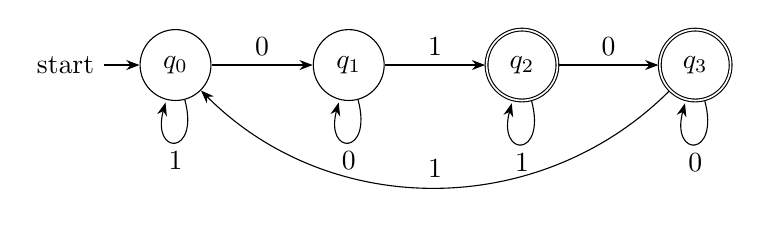
\begin{tikzpicture}[
    >=Stealth,
    node distance=2.2cm,
    on grid,
    auto,
    every state/.style={
        draw,
        circle,
        minimum size=0.9cm
    }
]

% states
\node[state, initial] (q0) {$q_0$};
\node[state, right=of q0] (q1) {$q_1$};
\node[state, accepting, right=of q1] (q2) {$q_2$};
\node[state, accepting, right=of q2] (q3) {$q_3$};

% transitions
\path[->]
(q0) edge node {$0$} (q1)
(q1) edge node {$1$} (q2)
(q2) edge node {$0$} (q3)

(q0) edge[loop below] node {$1$} ()
(q1) edge[loop below] node {$0$} ()
(q2) edge[loop below] node {$1$} ()
(q3) edge[loop below] node {$0$} ()

(q3) edge[bend left=45] node[above] {$1$} (q0);

\end{tikzpicture}
\end{center}
\subsubsection{NFA}
\[
NFA = (Q, \Sigma, \delta, q_0, F)
\]
\begin{flalign*}
Q &= \{q_0, q_1, q_2\cdots\} & \\
\Sigma &= \{a, b, c\cdots\} & \\
\delta &: Q \times \Sigma \to 2^Q = \{S | S \subseteq Q\} & \\
q_0 &\in Q(\text{一个开始状态}) & \\
F &\subseteq Q(\text{一个或多个接受状态}) &
\end{flalign*}
显而易见，每个DFA都是一个NFA。
\theorem{}{每一个NFA都可以转换成一个等价的DFA。}
\begin{proof}
设NFA为$N=(Q, \Sigma, \delta, q_0, F)$，我们构造一个DFA$D=(Q', \Sigma, \delta', q_0', F')$，其中：
\begin{itemize}
\item $Q' = 2^Q$，即DFA的状态集合是NFA状态集合的幂集。
\item $q_0' = \{q_0\}$，DFA的初始状态是NFA的初始状态的集合。
\item 对于每个状态集合$S \subseteq Q$和输入符号$a \in \Sigma$，定义$\delta'(S, a) = \bigcup_{q \in S} \delta(q, a)$，即DFA在状态集合$S$上输入符号$a$时转移到所有NFA状态$q$在输入符号$a$时转移的状态集合的并集。
\item $F' = \{S \subseteq Q | S \cap F \neq \emptyset\}$，DFA的接受状态集合是所有包含至少一个NFA接受状态的状态集合。
\end{itemize}
通过上述构造，我们可以证明DFA $D$接受的语言与NFA $N$接受的语言相同。对于任意输入字符串，DFA $D$在状态集合上进行转移，而NFA $N$在单个状态上进行转移。由于DFA $D$的状态集合包含了NFA $N$的所有可能状态，因此DFA $D$能够模拟NFA $N$的行为，并且接受相同的语言。
\end{proof}
NFA转化DFA例子：
这是一个NFA，接受语言$L$，其中
\[L=\{w \in \{0,1\}^* \mid w \text{ 以 }01\text{ 结尾}\}\]
\begin{center}
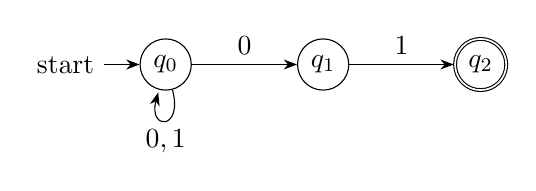
\begin{tikzpicture}[
    >=Stealth,
    node distance=2cm,
    on grid,
    auto,
    every state/.style={
        draw,
        circle,
        minimum size=0.65cm,
        inner sep=1pt
    }
]

\node[state, initial, initial text=start] (q0) {$q_0$};
\node[state, right=of q0] (q1) {$q_1$};
\node[state, accepting, right=of q1] (q2) {$q_2$};

\path[->]
(q0) edge node[above] {$0$} (q1)
(q1) edge node[above] {$1$} (q2)
(q0) edge[loop below] node {$0,1$} ();

\end{tikzpicture}
\end{center}

列出DFA所有可能状态集合：
\[
\begin{array}{|c|c|c|}
\hline
                     & 0                & 1                \\
\hline
\varnothing          & \varnothing      & \varnothing      \\
\hline
\{q_0\}              & \{q_0, q_1\}     & \{q_0\}          \\
\hline
\{q_1\}              & \varnothing      & \{q_2\}          \\
\hline
\{q_2\}              & \varnothing      & \varnothing      \\
\hline
\{q_0, q_1\}         & \{q_0, q_1\}     & \{q_0, q_2\}     \\
\hline
\{q_0, q_2\}         & \{q_0, q_1\}     & \{q_0\}          \\
\hline
\{q_1, q_2\}         & \varnothing      & \{q_2\}          \\
\hline
\{q_0, q_1, q_2\}    & \{q_0, q_1\}     & \{q_0, q_2\}     \\
\hline
\end{array}
\]
删除含有$\varnothing$的状态，删除不可达的状态，得到DFA状态转移表：
\[
\begin{array}{|c|c|c|c|}
\hline
\text{状态}            & 0                & 1                & \text{备注}      \\
\hline
A=\{q_0\}              & B                & A                & \text{初态}       \\
\hline
B=\{q_0, q_1\}         & B                & C                &                   \\
\hline
C=\{q_0, q_2\}         & B                & A                & \text{接受状态}    \\
\hline
\end{array}
\]
其中初态和NFA的初态相同，接受状态是所有包含NFA接受状态的状态集合。
构造DFA状态转移图：
\begin{center}
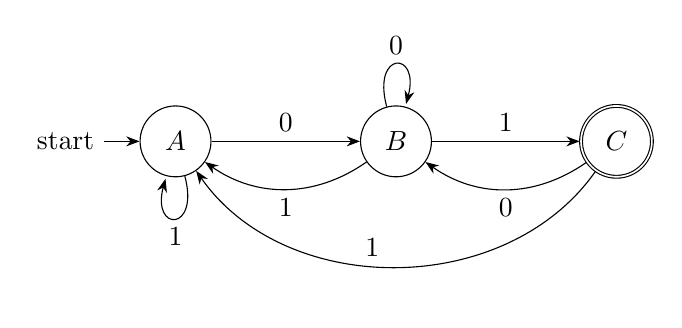
\begin{tikzpicture}[
    >=Stealth,
    node distance=2.8cm,
    on grid,
    auto,
    every state/.style={
        draw,
        circle,
        minimum size=0.9cm
    }
]

% states
\node[state, initial] (A) {$A$};
\node[state, right=of A] (B) {$B$};
\node[state, accepting, right=of B] (C) {$C$};

% transitions
\path[->]
(A) edge node[above] {$0$} (B)
(B) edge node[above] {$1$} (C)

(C) edge[bend left=35] node[below] {$0$} (B)
(B) edge[bend left=35] node[below] {$1$} (A)

(A) edge[loop below] node {$1$} ()
(B) edge[loop above] node {$0$} ()

(C) edge[bend left=55] node[above, pos=0.55] {$1$} (A);

\end{tikzpicture}
\end{center}


\subsubsection{$\varepsilon$-NFA}
\[
\varepsilon\text{-NFA} = (Q, \Sigma, \delta, q_0, F)
\]
\begin{flalign*}
Q &= \{q_0, q_1, q_2\cdots\} & \\
\Sigma &= \{a, b, c\cdots\} & \\
\delta &: Q \times (\Sigma \cup \{\varepsilon\}) \to 2^Q & \\
q_0 &\in Q(\text{一个开始状态}) & \\
F &\subseteq Q(\text{一个或多个接受状态}) &
\end{flalign*}
此后除非特别申明，不再明确区分$\varepsilon$-NFA和NFA, 而是都称为NFA。
\subsubsection{状态的$\varepsilon$-闭包}
状态q的$\varepsilon$-闭包是指从状态q出发，通过$\varepsilon$转移可以到达的所有状态的集合，记为$ECLOSE(q)$。
递归定义如下：
\begin{itemize}
\item $q \in ECLOSE(q)$
\item $\forall p \in ECLOSE(q), \forall r \in \delta(p, \varepsilon), r \in ECLOSE(q)$
\end{itemize}
相应状态集的$\varepsilon$-闭包定义为
\[
ECLOSE(S) = \bigcup_{q \in S} ECLOSE(q)
\]
\subsubsection{扩展转移函数}
对于NFA $N=(Q, \Sigma, \delta, q_0, F)$，定义扩展转移函数$\hat{\delta}: Q \times \Sigma^* \to 2^Q$如下：
\begin{itemize}
\item $\hat{\delta}(q, \varepsilon) = ECLOSE(q)$
\item $\hat{\delta}(q, wa) = \bigcup_{p \in \hat{\delta}(q, w)} ECLOSE(\delta(p, a))$，其中$w \in \Sigma^*$，$a \in \Sigma$。
即是$\hat{\delta}(q, w)$的可达状态集合
\end{itemize}
\theorem{}{每一个$\varepsilon$-NFA都可以转换成一个等价的DFA。}
\begin{proof}
设$\varepsilon$-NFA为$N=(Q, \Sigma, \delta, q_0, F)$，我们构造一个DFA$D=(Q', \Sigma, \delta', q_0', F')$，其中：
\begin{itemize}
\item $Q' = 2^Q$，即DFA的状态集合是NFA状态集合的幂集。
\item $q_0' = ECLOSE(q_0)$，DFA的初始状态是NFA的初始状态的$\varepsilon$-闭包。
\item 对于每个状态集合$S \subseteq Q$和输入符号$a \in \Sigma$，定义$\delta'(S, a) = \bigcup_{q \in S} ECLOSE(\delta(q, a))$，即DFA在状态集合$S$上输入符号$a$时转移到所有NFA状态$q$在输入符号$a$时转移的状态集合的$\varepsilon$-闭包的并集。
\item $F' = \{S \subseteq Q | S \cap F \neq \emptyset\}$，DFA的接受状态集合是所有包含至少一个NFA接受状态的状态集合。
\end{itemize}
\end{proof}
$\varepsilon$-NFA到DFA的转换例子：
这是一个$\varepsilon$-NFA，接受语言$L$，其中
\[L=\{w \in \{0,1\}^* \mid w \text{ 以 }01\text{ 结尾}\}\]
\begin{center}
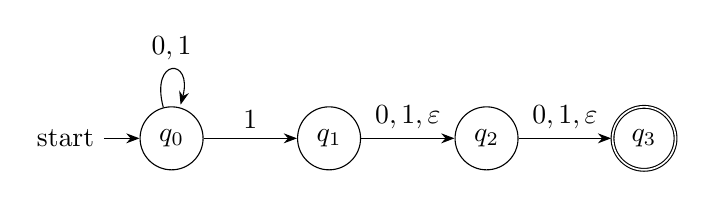
\begin{tikzpicture}[
    >=Stealth,
    node distance=2cm,
    on grid,
    auto,
    every state/.style={
        draw,
        circle,
        minimum size=0.8cm
    }
]

% states
\node[state, initial, initial text=start] (q0) {$q_0$};
\node[state, right=of q0] (q1) {$q_1$};
\node[state, right=of q1] (q2) {$q_2$};
\node[state, accepting, right=of q2] (q3) {$q_3$};

% transitions
\path[->]
(q0) edge[loop above] node {$0,1$} ()
(q0) edge node[above] {$1$} (q1)
(q1) edge node[above] {$0,1,\varepsilon$} (q2)
(q2) edge node[above] {$0,1,\varepsilon$} (q3);

\end{tikzpicture}
\end{center}
列出DFA所有可能状态集合：
\[
\begin{array}{|c|c|c|}
\hline
                                & 0                      & 1                      \\
\hline
\varnothing                     & \varnothing            & \varnothing            \\
\hline
\{q_0\}                         & \{q_0\}                & \{q_0, q_1, q_2, q_3\} \\
\hline
\{q_1\}                         & \{q_2, q_3\}           & \{q_2, q_3\}           \\
\hline
\{q_2\}                         & \{q_3\}                & \{q_3\}                \\
\hline
\{q_3\}                         & \varnothing            & \varnothing            \\
\hline
\{q_0, q_1\}                    & \{q_0, q_2, q_3\}      & \{q_0, q_1, q_2, q_3\} \\
\hline
\{q_0, q_2\}                    & \{q_0, q_3\}           & \{q_0, q_1, q_2, q_3\} \\
\hline
\{q_0, q_3\}                    & \{q_0\}                & \{q_0, q_1, q_2, q_3\} \\
\hline
\{q_1, q_2\}                    & \{q_2, q_3\}           & \{q_2, q_3\}           \\
\hline
\{q_1, q_3\}                    & \{q_2, q_3\}           & \{q_2, q_3\}           \\
\hline
\{q_2, q_3\}                    & \{q_3\}                & \{q_3\}                \\
\hline
\{q_0, q_1, q_2\}               & \{q_0, q_2, q_3\}      & \{q_0, q_1, q_2, q_3\} \\
\hline
\{q_0, q_1, q_3\}               & \{q_0, q_2, q_3\}      & \{q_0, q_1, q_2, q_3\} \\
\hline
\{q_0, q_2, q_3\}               & \{q_0, q_3\}           & \{q_0, q_1, q_2, q_3\} \\
\hline
\{q_1, q_2, q_3\}               & \{q_2, q_3\}           & \{q_2, q_3\}           \\
\hline
\{q_0, q_1, q_2, q_3\}          & \{q_0, q_2, q_3\}      & \{q_0, q_1, q_2, q_3\} \\
\hline
\end{array}
\]
删除含有$\varnothing$的状态，删除不可达的状态，得到DFA状态转移表：
\[
\begin{array}{|c|c|c|c|}
\hline
\text{状态}                        & 0                & 1                & \text{备注}      \\
\hline
A=\{q_0\}                          & A                & B                & \text{初态}       \\
\hline
B=\{q_0, q_1, q_2, q_3\}           & C                & B                & \text{接受状态}    \\
\hline
C=\{q_0, q_2, q_3\}                & D                & B                & \text{接受状态}    \\
\hline
D=\{q_0, q_3\}                     & A                & B                & \text{接受状态}    \\
\hline
\end{array}
\]
构造DFA状态转移图：
\begin{center}
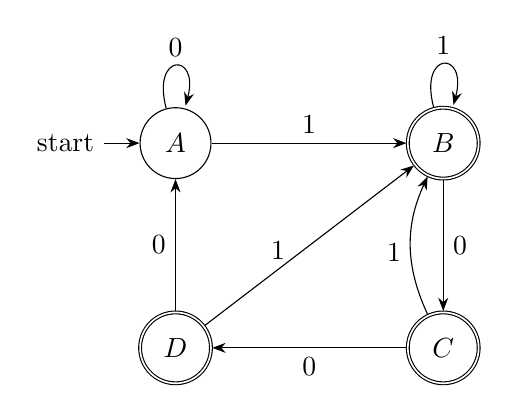
\begin{tikzpicture}[
    >=Stealth,
    node distance=2.6cm and 3.4cm,
    on grid,
    auto,
    every state/.style={
        draw,
        circle,
        minimum size=0.9cm
    }
]

% states
\node[state, initial] (A) {$A$};
\node[state, accepting, right=of A] (B) {$B$};
\node[state, accepting, below=of B] (C) {$C$};
\node[state, accepting, below=of A] (D) {$D$};

% transitions
\path[->]
% square edges
(A) edge node[above] {$1$} (B)
(B) edge node[right] {$0$} (C)
(C) edge node[below] {$0$} (D)
(D) edge node[left] {$0$} (A)

% loops
(A) edge[loop above] node {$0$} ()
(B) edge[loop above] node {$1$} ()

% C -> B, slightly curved to avoid B -> C
(C) edge[bend left=25] node[left, pos=0.45] {$1$} (B)

% D -> B, route outside
(D) edge node[pos=0.35, above] {$1$} (B);

\end{tikzpicture}
\end{center}
例题：设计一个$\varepsilon$-NFA，接受语言$L$，其中
\[L=\{w | w \in \{a,b,c\}^*\wedge w\text{的前5位至少有一个子串bac} \wedge 
w\text{的后5位至少有一个子串acb}\}\]
\subsection{上下文有关文法}
\subsection{短语文法}
\end{document}